\documentclass[11pt,english]{article}
\usepackage[a4paper,
            bindingoffset=0.2in,
            left=0.5in,
            right=0.5in,
            top=0.5in,
            bottom=0.5in,
            footskip=.25in]{geometry}
\usepackage[utf8]{inputenc}
\usepackage[english]{babel}
\usepackage{biblatex}
\addbibresource{citations.bib}
\usepackage{csquotes}
\usepackage{fancyhdr}
\usepackage{longtable}
\usepackage{multirow}
\usepackage{graphicx}

\usepackage[automake]{glossaries} %Load glossaries package
\makeglossaries
\pagestyle{fancy}
\title{Medical Image Registration}
\author{Mudalige Dineth Navodya\\170401V}
\date{\today}
\pagestyle{fancy}
\rhead{170401V}
\lhead{BM4301 - Medical Image Processing}
\rfoot{\title}
\begin{document}
\maketitle
\thispagestyle{fancy}
\printglossary[title={List of Abbreviations}] %Generate List of Abbreviations



\newglossaryentry{ITK}{name={ITK},description={Insight Toolkit}}
\newglossaryentry{L-BFGS}{name={L-BFGS},description={Limited memory Broyden, Fletcher, Goldfarb, Shannon, Bound Constrained}}
\newglossaryentry{MRI}{name={MRI},description={Magnetic Resonance Imaging}}

\section*{Introduction}
Registration is the aligning of the target with the source. It can be mathematically explained as finding the spatial transform that maps points from one image to a homologous points on a object in the second image\cite{itkmanual2}.\\
Registration is a non-linear optimization method. As any optimization method, it needs an initial transformation as the intial estimate\cite{overview}. In \gls{ITK}, there is a registration framework shown in Figure[\ref{fig:framework}] to standardize the registration process.
\section*{Registration Framework\cite{itkmanual2}}
The basic data to the registration framework are two images.  
\begin{enumerate}
    \item Fixed Image(f(x))
    \item Moving image(m(x))
\end{enumerate}
This provides more flexibility because the registration computations can happen on a physical grid completely different the fixed image domain having different sampling density. 
\begin{figure}[h!]
    \centering
    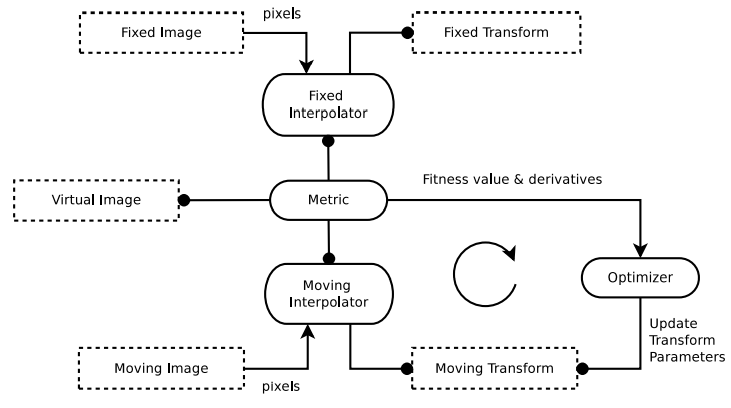
\includegraphics[width =0.6\textwidth] {images/framework.PNG}
    \caption{ITKv4 registration framework\cite{itkmanual2}}
    \label{fig:framework}
\end{figure}
The main components in the registration framework are as follows.
\begin{enumerate}
    \item Transform - Spatial mapping needed to map the points from one domain to another domain
    \item Interpolator - Evaluates the image intensities at each point in the virtual space
    \item Similarity metric - Measure of how well an image is matched by the transformed image. This is the key component that controls the registration process.
    \item Optimizer - Updates the parameters based on the outputs of the cost function
\end{enumerate}
\section*{Methodology}
After loading the images, the registration framework is applied to the images. The most important part is to select the ideal transform or function to be used as the main components of the framework.  
\subsection*{Visualization}
The two images are visualized initially and they are placed one over another using alpha blending. Alpha blending is used to combine the two images in such a manner that both images are visible in the single image.  
\begin{figure}[h!]
    \centering
    \begin{minipage}[b]{0.6\textwidth}
      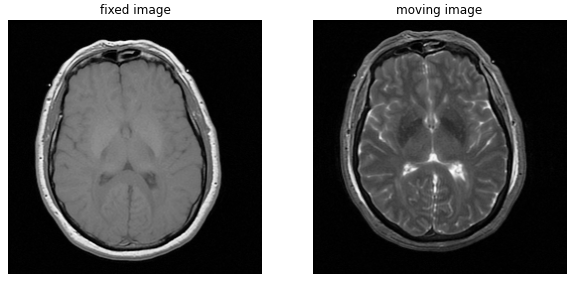
\includegraphics[width = \textwidth]{images/initial.PNG}
      \caption{Slice 16 of Fixed and Moving Images}
      \label{fig:initial}
    \end{minipage}
    \begin{minipage}[b]{0.3\textwidth}
      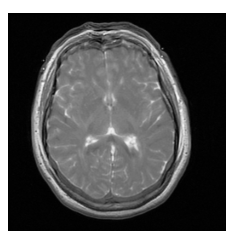
\includegraphics[width = \textwidth]{images/initialOverlap.PNG}
      \caption{Slice 16 of overlapped image($\alpha=0.5$)}
      \label{fig:czchirp100}
    \end{minipage}
  \end{figure}
From Figure[\ref{fig:initial}], it is clear that the two images have differences in intensities and position. The change of the position is clear with the overlapped image shown in Figure[\ref{fig:czchirp100}].
\subsection*{Selection of Intial Transform}
Due to the need of an initial estimate for optimization, an initial transform is used. There are two options for initialization\cite{overview}.
\begin{enumerate}
    \item Identity transform - This is when no initialization is used. 
    \item CenteredTransformInitializerFilter - This aligns the physical centers of the two images
\end{enumerate}
By looking at the two images it can be assumed that a translation transform will be sufficient as the initial transform because the orientation shown in both images is the same visibly there is a difference in the placement of the two images. To be sure about the behaviours of the transforms several transforms available in the \gls{ITK} registration framework are tested for these images with a Linear interpolator, Gradient Descent optimizer and Mattes Mattes Mutual Information metric.
\begin{longtable}[c]{|l|c|c|}
    \caption{Comparison of various transforms}
    \label{tab:transform}\\
    \hline
    \multicolumn{1}{|c|}{\textbf{Transform}}                                    & \textbf{Metric} & \textbf{Iterations} \\ \hline
    \endfirsthead
    %
    \endhead
    %
    \textbf{\begin{tabular}[c]{@{}l@{}}Identity\\ (Nothing done)\end{tabular}}  & -0.47915        & 31                  \\ \hline
    \textbf{\begin{tabular}[c]{@{}l@{}}Centered Geometry\\ Euler3D\end{tabular}} & -0.35996 & 29 \\ \hline
    \textbf{\begin{tabular}[c]{@{}l@{}}Centered Moments\\ Euler3D\end{tabular}} & -0.72910        & 9                   \\ \hline
    \textbf{\begin{tabular}[c]{@{}l@{}}Centered\\ VersorRigid3D\end{tabular}}   & -0.68326        & 10                  \\ \hline
    \textbf{Translation}                                                        & -0.68272        & 10                  \\ \hline
    \end{longtable}
    \begin{figure}[h!]
        \centering
        \begin{minipage}[b]{0.2\textwidth}
          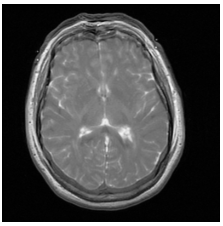
\includegraphics[width = \textwidth]{images/identityOverlap.PNG}
          \caption{Slice 16 of Identity Transform}
          \label{fig:identity}
        \end{minipage}
        \begin{minipage}[b]{0.2\textwidth}
          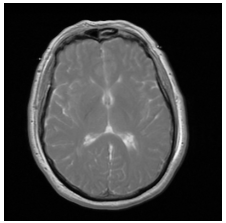
\includegraphics[width = \textwidth]{images/versorOverlap.PNG}
          \caption{Slice 16 of VersorRigid3D Transform}
          \label{fig:versor}
        \end{minipage}
        \begin{minipage}[b]{0.2\textwidth}
            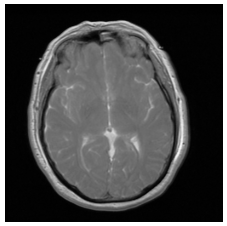
\includegraphics[width = \textwidth]{images/translationOverlap.PNG}
            \caption{Slice 16 of Translation Transform}
            \label{fig:translation}
          \end{minipage}
          \begin{minipage}[b]{0.2\textwidth}
            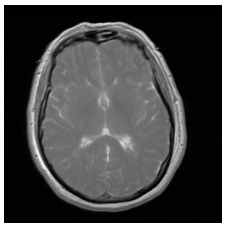
\includegraphics[width = \textwidth]{images/centeredMomentOverlap.PNG}
            \caption{Slice 16 of Euler3D Moments Transform}
            \label{fig:euler3D}
          \end{minipage}
      \end{figure}
\subsection*{Selection of Interpolator}
Normally, the interpolator is used is the Linear interpolator but the registration can be improved with the use of other interpolators as well.  
\begin{longtable}[c]{|l|l|c|c|}
    \caption{Comparison of Interpolators}
    \label{tab:interpolator}\\
    \hline
    \textbf{Transform} &
      \multicolumn{1}{c|}{\textbf{Interpolator}} &
      \textbf{Metric} &
      \textbf{Iterations} \\ \hline
    \endfirsthead
    %
    \endhead
    %
    \multirow{6}{*}{\textbf{\begin{tabular}[c]{@{}l@{}}Centered Moment\\ Euler 3D\end{tabular}}} &
      Nearest Neighbour &
      -0.05969 &
      9 \\ \cline{2-4} 
                                          & Gaussian                                                         & -0.68382 & 11 \\ \cline{2-4} 
                                          & \begin{tabular}[c]{@{}l@{}}Hamming Windowed\\ Sinc\end{tabular}  & -0.68321 & 10 \\ \cline{2-4} 
                                          & \begin{tabular}[c]{@{}l@{}}Cosined Windowed\\ Sinc\end{tabular}  & -0.66679 & 10 \\ \cline{2-4} 
                                          & \begin{tabular}[c]{@{}l@{}}Lanczos Windowed\\ Sinc\end{tabular}  & -0.65813 & 9  \\ \cline{2-4} 
                                          & \begin{tabular}[c]{@{}l@{}}Blackman Windowed\\ Sinc\end{tabular} & -0.64670 & 9  \\ \hline
    \multirow{6}{*}{\textbf{\begin{tabular}[c]{@{}l@{}}Centered\\ VersorRigid3D\end{tabular}}} &
      \begin{tabular}[c]{@{}l@{}}Blackman Windowed\\ Sinc\end{tabular} &
      -0.71825 &
      10 \\ \cline{2-4} 
                                          & \begin{tabular}[c]{@{}l@{}}Lanczos Windowed\\ Sinc\end{tabular}  & -0.69272 & 10 \\ \cline{2-4} 
                                          & \begin{tabular}[c]{@{}l@{}}Cosine Windowed\\ Sinc\end{tabular}   & -0.67357 & 10 \\ \cline{2-4} 
                                          & \begin{tabular}[c]{@{}l@{}}Hamming Windowed\\ Sinc\end{tabular}  & -0.67180 & 9  \\ \cline{2-4} 
                                          & Gaussian                                                         & -0.76092 & 9  \\ \cline{2-4} 
                                          & Nearest Neighbour                                                & -0.63662 & 9  \\ \hline
    \multirow{2}{*}{\textbf{Translation}} & Gaussian                                                         & -0.75211 & 10 \\ \cline{2-4} 
                                          & \begin{tabular}[c]{@{}l@{}}Blackman Windowed\\ Sinc\end{tabular} & -0.65999 & 10 \\ \hline
    \end{longtable}
    From the Table[\ref{tab:interpolator}], it is clear that Gaussian interpolator performs better with VersorRigid3D and Translation transforms. 
    \pagebreak
    \begin{figure}[h!]
        \centering
        \begin{minipage}[b]{0.3\textwidth}
            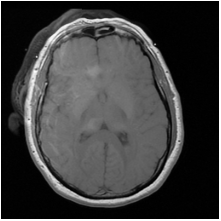
\includegraphics[width = \textwidth]{images/eulerNN.PNG}
            \caption{Euler3D with NearestNeighbour}
            \label{fig:eulerNN}
          \end{minipage}
        \begin{minipage}[b]{0.3\textwidth}
          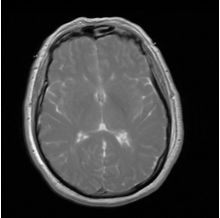
\includegraphics[width = \textwidth]{images/versorGaussian.PNG}
          \caption{VersorRigid3D with Gaussian}
          \label{fig:verserGaussian}
        \end{minipage}
        \begin{minipage}[b]{0.3\textwidth}
            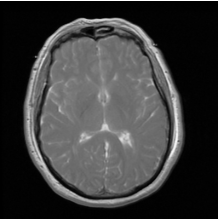
\includegraphics[width = \textwidth]{images/translationGaussian.PNG}
            \caption{Translation with Gaussian}
            \label{fig:translationGaussian}
          \end{minipage}
      \end{figure}
From the Figure[\ref{fig:eulerNN}], it is clear that if the interpolator is not properly chosen it will degrade the results of the initial transform. A correct selection of the interpolator will improve the results of the initial transform as shown in Figure[\ref{fig:translationGaussian}] and Figure[\ref{fig:verserGaussian}].    
\subsection*{Selection of Optimizer}
Optimizer will guarantee the convergence of the registration and conserve the time taken for the output. There are two types of optimizers. 
\begin{enumerate}
    \item Gradient Based 
    \begin{itemize}
        \item Exhaustive 
        \item One Plus One evolutionary optimizer  
    \end{itemize}
    \item Non-gradient based 
    \begin{itemize}
        \item Gradient Descent  
        \item Gradient Descent Line Search  
        \item \gls{L-BFGS}
    \end{itemize}
From Table[\ref{tab:optimizers}] it is clear that the non-gradient based optimizers do not work properly when compared to the gradient based optimizers. Therefore, a better optimization is guaranteed with gradient based optimizers.\\  
One plus one evolutionary optimizer uses the biological evolution of samples. This is used for bias correction in \gls{MRI}\cite{itkmanual2}.\gls{L-BFGS} is a better optimizer because it is a true quasi-Newton method. In a parameter space with flat valleys,\gls{L-BFGS} performs well. The downside is that it calculates the Hessian approximation in every step leading to long run times. But in a scenario like an image with limited data \gls{L-BFGS} performs better\cite{LBFGS}.
\end{enumerate}
\begin{longtable}[c]{|l|l|c|c|}
    \caption{Comparison of optimizers}
    \label{tab:optimizers}\\
    \hline
    \textbf{Transform} &
      \textbf{Optimizer} &
      \multicolumn{1}{l|}{\textbf{Metric}} &
      \multicolumn{1}{l|}{\textbf{Iterations}} \\ \hline
    \endfirsthead
    %
    \endhead
    %
    \multirow{3}{*}{VersorRigid3D} &
      \begin{tabular}[c]{@{}l@{}}GradientDescent\\ Line Search\end{tabular} &
      -0.63509 &
      31 \\ \cline{2-4} 
                & OnePlusOne  & -0.62899 & Over 100 \\ \cline{2-4} 
                & \gls{L-BFGS} & -0.83929 & Over 100 \\ \hline
    Translation & \gls{L-BFGS} & -0.84056 & Over 100 \\ \hline
\end{longtable}
\begin{figure}[h!]
    \centering
    \begin{minipage}[b]{0.3\textwidth}
        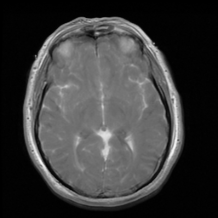
\includegraphics[width = \textwidth]{images/versorOnePlusOne.PNG}
        \caption{VersorRigid3D with OneplusOne}
        \label{fig:versor1plus1}
      \end{minipage}
    \begin{minipage}[b]{0.3\textwidth}
      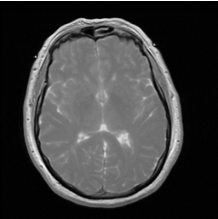
\includegraphics[width = \textwidth]{images/VersorLBFGS.PNG}
      \caption{VersorRigid3D with \gls{L-BFGS}}
      \label{fig:versorLBFGS}
    \end{minipage}
    \begin{minipage}[b]{0.3\textwidth}
        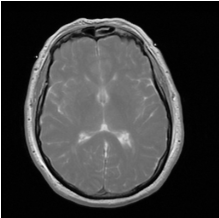
\includegraphics[width = \textwidth]{images/TranslationLBFGS.PNG}
        \caption{Translation with \gls{L-BFGS}}
        \label{fig:translationLBFGS}
      \end{minipage}
  \end{figure}
\subsection*{Selection of metric}
All the metrics used in the registration framework minimizes when the optimization problem converges. Therefore, the selection of the metric is not that crucial. The Mattes Mutual Information metric can be calculated fast and it is normally used.
\section*{Results}
It can be concluded from the results in Tables \ref{tab:interpolator},\ref{tab:transform} and \ref{tab:optimizers}, that the most optimum selection of the main components of the registration framework can be listed as follows. 
\begin{itemize}
    \item Transform - Translation Transform  
    \item Interpolator - Gaussian Interpolator
    \item Optimizer - \gls{L-BFGS}
    \item Metric - Mattes Mutual Information
\end{itemize}
\begin{figure}[h!]
    \centering
    \begin{minipage}[b]{0.22\textwidth}
        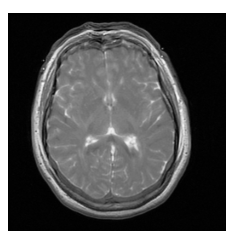
\includegraphics[width = \textwidth]{images/initialOverlap.PNG}
        \caption{Slice 16 of initial images}
        \label{fig:initialOverlap}
      \end{minipage}
    \begin{minipage}[b]{0.22\textwidth}
      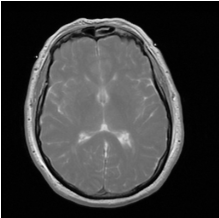
\includegraphics[width = \textwidth]{images/TranslationLBFGS.PNG}
      \caption{Slice 16 of best registration}
      \label{fig:versor1LBFGS}
    \end{minipage}
    \begin{minipage}[b]{0.22\textwidth}
        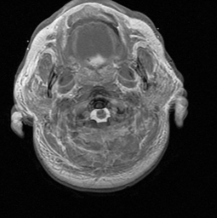
\includegraphics[width = \textwidth]{images/lastInitial.PNG}
        \caption{Slice 32 of initial images}
        \label{fig:initiallastOverlap}
      \end{minipage}
    \begin{minipage}[b]{0.22\textwidth}
      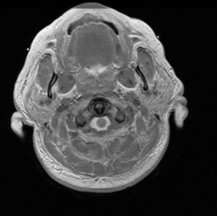
\includegraphics[width = \textwidth]{images/lastTranslation.PNG}
      \caption{Slice 32 of best registration}
      \label{fig:versorlastLBFGS}
    \end{minipage}
  \end{figure}
\printbibliography
\end{document}
